
Системийн үйл ажилгааны загвар нь хэрэглэгчид (Администратор, Менежер, Ажилтан) болон системийн хоорондын харилцан үйлчлэлийг харуулна. Энэхүү диаграмм нь системийн үндсэн функцуудыг тодорхойлж, хэрэглэгч тус бүр ямар үйлдэл гүйцэтгэх боломжтойг илэрхийлнэ. Доорх Хүснэгт 3.5-д хэрэглээний хувилбаруудыг дүрслэн харуулав.

\begin{figure}[h!]
    \centering
    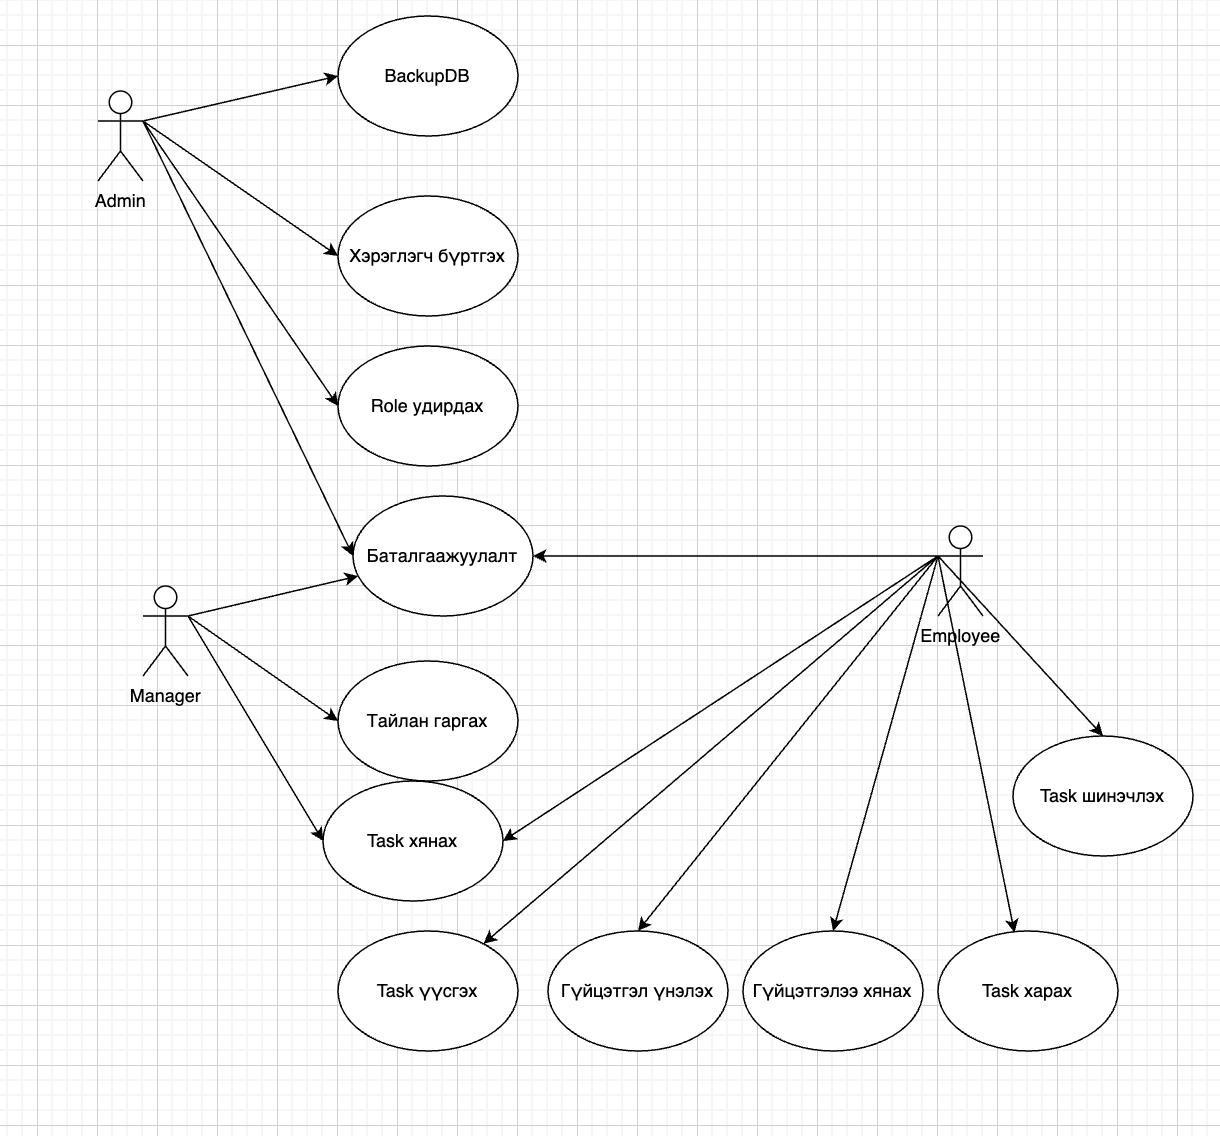
\includegraphics[width=\textwidth]{src/images/usecase-diagram.png}
    \caption{Ажилтны Гүйцэтгэлийн Үнэлгээний Системийн Үйл Ажилгааны Загвар}
    \label{fig:usecase_diagram}
\end{figure}

\textbf{Тайлбар:} Хүснэгт 3.5-д администратор хэрэглэгчдийг бүртгэх, эрх удирдах зэрэг үйлдэл хийдэг бол менежер даалгавар хуваарилах, гүйцэтгэлийг үнэлэх, ажилтан өөрийн даалгавар болон гүйцэтгэлийг хянах боломжтой гэдгийг харуулсан. Нэвтрэлтийн баталгаажуулалт нь бүх хэрэглэгчдэд хамаатай бөгөөд JWT технологи ашиглана.
\pagebreak